\documentclass[../TDON2_inter.tex]{subfiles}%

\begin{document}
\section[s]"1"{Contrôle actif du bruit en conduite}

\enonce{%
	\noindent
	\begin{minipage}{0.70\linewidth}
		On s'intéresse à un système conçu pour l'élimination d'un bruit in-
		désirable transporté par une conduite. Le bruit est détecté par un premier
		micro dont le signal est reçu par un contrôleur électronique. Le contrôleur,
		qui est le centre du système, envoie sur un haut-parleur la tension adéquate
		pour générer une onde de signal exactement opposé à celui du bruit de
		manière à ce que l'onde résultante au point A (voir figure ci-contre) et
		au-delà de A soit nulle.
	\end{minipage}
	\hfill
	\begin{minipage}{0.30\linewidth}
		\begin{center}
			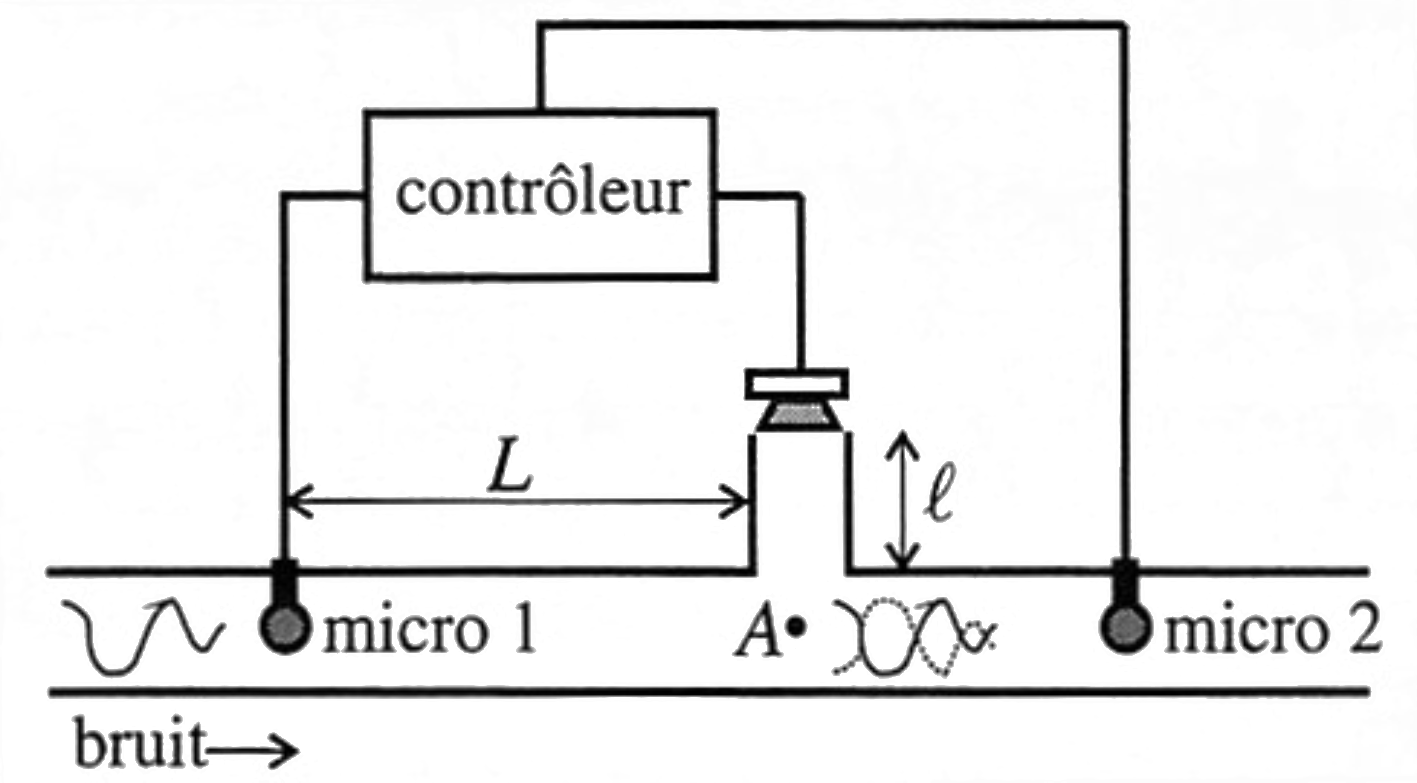
\includegraphics[width=\linewidth]{conduite-plain_white}
		\end{center}
	\end{minipage}
}

\QR{%
	Exprimer, en fonction de $L$, $l$ et de la célérité $c$ du son, le
	temps disponible pour le calcul du signal envoyé sur le haut-parleur.
}{%
	Entre l'instant où le signal est détecté par le micro 1 et l'instant
	où ce signal passe en A, il s'écoule un temps égal à $L/c$. Pendant ce
	temps, il faut que le contrôleur calcule et produise le signal qu'il
	envoie dans le haut-parleur, et que ce signal se propage jusqu'à A, ce
	qui prend le temps $\ell/c$. Ainsi, le temps disponible pour le calcul
	est
	\[\boxed{\frac{L-\ell}{c}}\]
}

\QR{%
	On suppose le bruit sinusoïdal de pulsation $\omega$. On appelle
	$\f_1$ la phase initiale du signal détecté par le micro 1 et $\f_{\rm
			HP}$ la phase initiale du signal émis par le haut-parleur. Exprimer, en
	fonction de $\omega$, $c$, $L$ et $l$, la valeur que doit avoir $\D\f =
		\f_{\rm HP} - \f_1$
}{%
	La phase du signal de bruit arrivant en A est
	\[
		\f_{\rm bruit} = \f_1-kL
	\]
	La phase du signal de correction arrivant en A est
	\[
		\f_{\rm corr} = \f_{\rm HP} -k\ell
	\]
	Pour avoir interférences destructives, il faut que $\f_{\rm corr} =
		\f_{\rm bruit} + \pi$, c'est-à-dire
	\[
		\boxed{\D\f_{c/b}({\rm A})
			= \f_{\rm HP} - \f_1
			= \frac{\w}{c}(\ell-L)+\pi}
	\]
}

\QR{%
	L'onde émise par le haut-parleur se propage dans la conduite dans les
	deux sens à partir de A. Expliquer l'utilité du micro 2.
}{%
	Le micro 1 capte un signal qui est la superposition du bruit et du
	signal émis par le haut-parleur se propageant à partir de A vers
	l'amont. Le micro 2 donne un contrôle du résultat et permet la
	détermination du meilleur signal de correction.
}
\end{document}
